\section{Mathematische Grundlagen}

\textbf{Kinematik} ist die reine geometrische Beschreibung von Bewegung eines Manipulators
oder Roboters. Das essentielle Konzept ist die \textbf{Position}.

\textbf{Statik} behandelt Kräfte und Momente, die sich auf einen ruhenden Mechanismus
auswirken. Das essentielle Konzept ist die \textbf{Steifigkeit}.

\textbf{Dynamik} analysiert die Kräfte und Momente, die durch Bewegung und Beschleunigung
eines Mechanismus und einer zusätzlichen Last entstehen.

\textbf{Terminologie}:
\begin{center}
	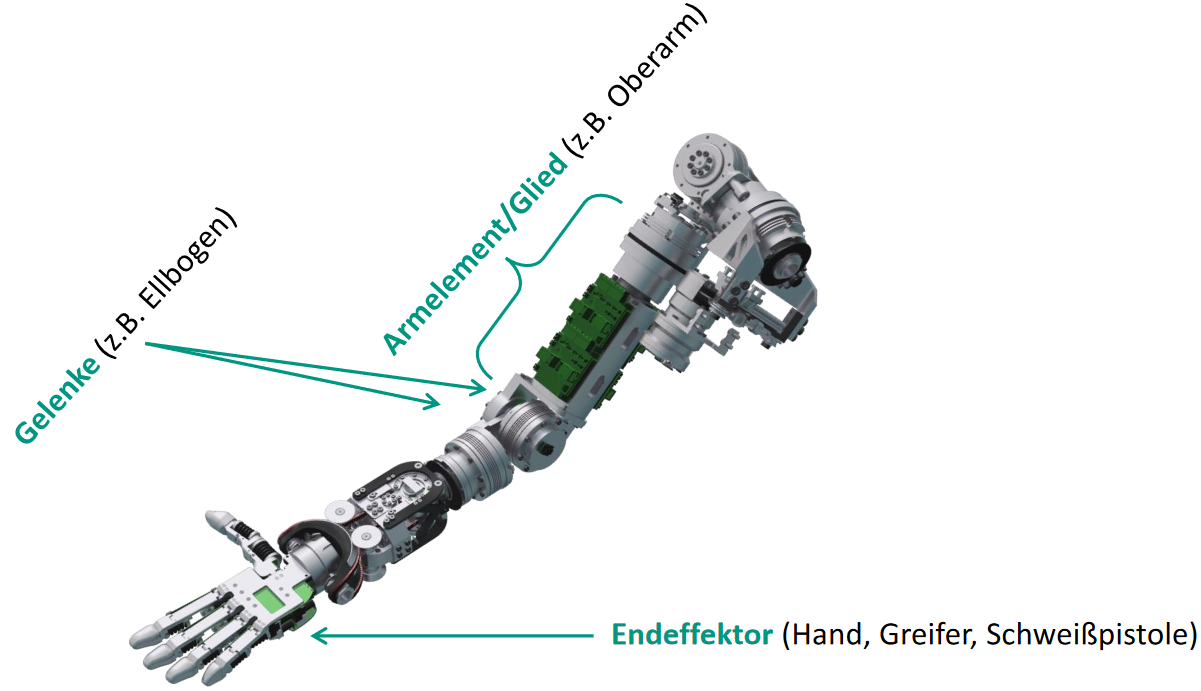
\includegraphics[width=0.7\textwidth]{images/arm.png}
\end{center}
\medskip
\textbf{Kinematische Kette} ist eine Menge an Gliedern, die durch Gelenke verbunden sind.

\textbf{Freiheitsgrade} (DoF) ist die Anzahl unabhängiger Parameter, die zur kompletten Spezifikation der Lage eines Objekts benötigt werden, z.B. Starrkörper hat in 2D 3 DoF und in 3D 6 DoF.

Starrkörperbewegungen werden durch zwei Eigenschaften charakterisiert:
\begin{enumerate}
	\item Distanz zweier beliebiger Punkte ist konstant
	\item Orientierungen im Körper bleiben erhalten
\end{enumerate}



